% Created by tikzDevice version 0.11 on 2018-04-09 15:27:50
% !TEX encoding = UTF-8 Unicode
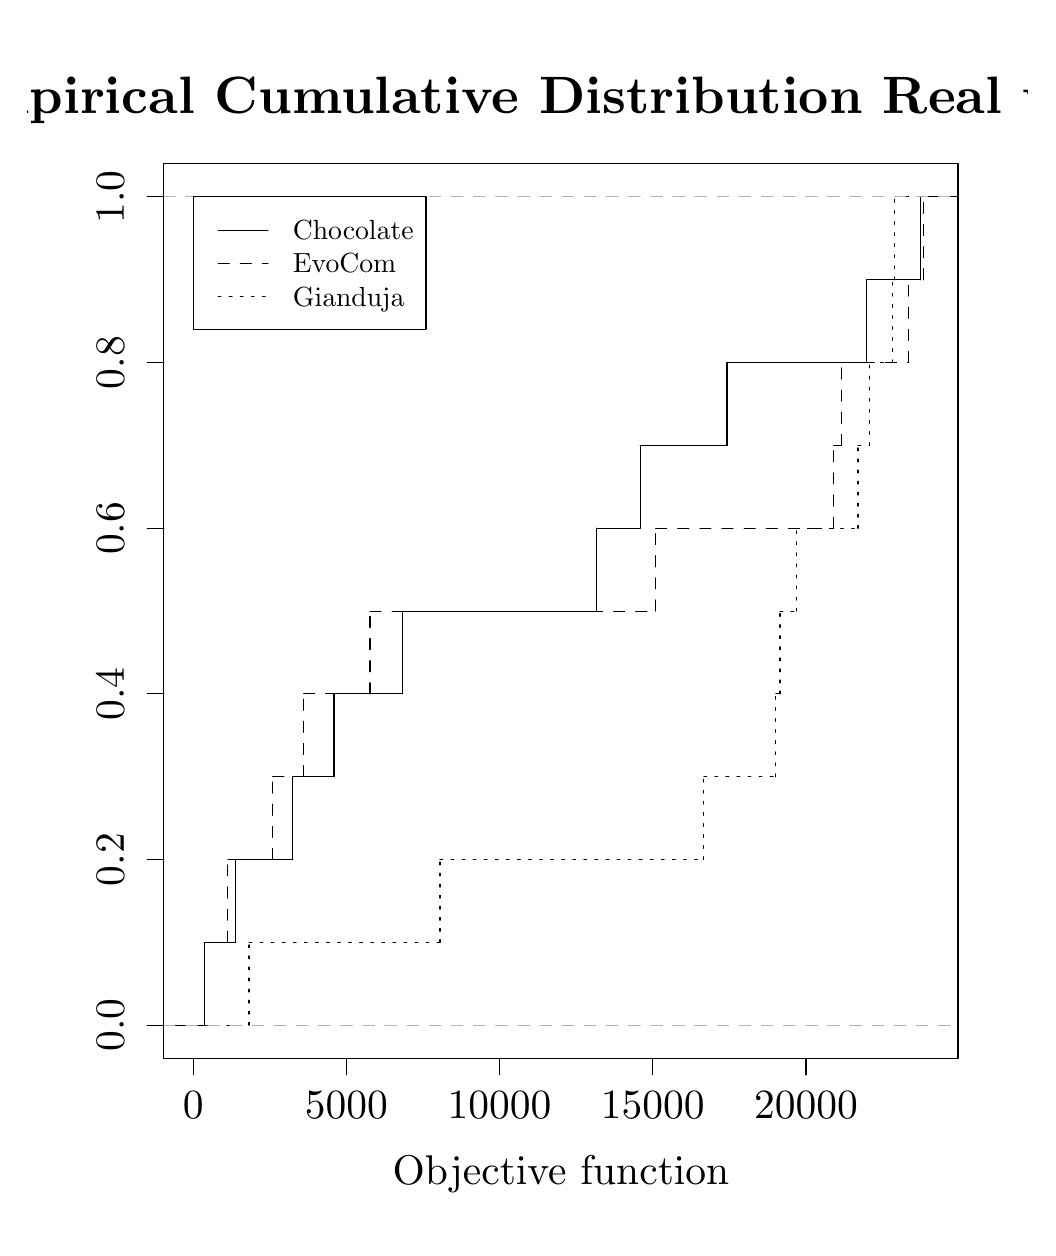
\begin{tikzpicture}[x=1pt,y=1pt]
\definecolor{fillColor}{RGB}{255,255,255}
\path[use as bounding box,fill=fillColor,fill opacity=0.00] (0,0) rectangle (361.35,433.62);
\begin{scope}
\path[clip] (  0.00,  0.00) rectangle (361.35,433.62);
\definecolor{drawColor}{RGB}{0,0,0}

\path[draw=drawColor,line width= 0.4pt,line join=round,line cap=round] ( 59.83, 61.20) -- (281.24, 61.20);

\path[draw=drawColor,line width= 0.4pt,line join=round,line cap=round] ( 59.83, 61.20) -- ( 59.83, 55.20);

\path[draw=drawColor,line width= 0.4pt,line join=round,line cap=round] (115.18, 61.20) -- (115.18, 55.20);

\path[draw=drawColor,line width= 0.4pt,line join=round,line cap=round] (170.53, 61.20) -- (170.53, 55.20);

\path[draw=drawColor,line width= 0.4pt,line join=round,line cap=round] (225.89, 61.20) -- (225.89, 55.20);

\path[draw=drawColor,line width= 0.4pt,line join=round,line cap=round] (281.24, 61.20) -- (281.24, 55.20);

\node[text=drawColor,anchor=base,inner sep=0pt, outer sep=0pt, scale=  1.50] at ( 59.83, 39.60) {0};

\node[text=drawColor,anchor=base,inner sep=0pt, outer sep=0pt, scale=  1.50] at (115.18, 39.60) {5000};

\node[text=drawColor,anchor=base,inner sep=0pt, outer sep=0pt, scale=  1.50] at (170.53, 39.60) {10000};

\node[text=drawColor,anchor=base,inner sep=0pt, outer sep=0pt, scale=  1.50] at (225.89, 39.60) {15000};

\node[text=drawColor,anchor=base,inner sep=0pt, outer sep=0pt, scale=  1.50] at (281.24, 39.60) {20000};

\path[draw=drawColor,line width= 0.4pt,line join=round,line cap=round] ( 49.20, 73.17) -- ( 49.20,372.45);

\path[draw=drawColor,line width= 0.4pt,line join=round,line cap=round] ( 49.20, 73.17) -- ( 43.20, 73.17);

\path[draw=drawColor,line width= 0.4pt,line join=round,line cap=round] ( 49.20,133.03) -- ( 43.20,133.03);

\path[draw=drawColor,line width= 0.4pt,line join=round,line cap=round] ( 49.20,192.88) -- ( 43.20,192.88);

\path[draw=drawColor,line width= 0.4pt,line join=round,line cap=round] ( 49.20,252.74) -- ( 43.20,252.74);

\path[draw=drawColor,line width= 0.4pt,line join=round,line cap=round] ( 49.20,312.59) -- ( 43.20,312.59);

\path[draw=drawColor,line width= 0.4pt,line join=round,line cap=round] ( 49.20,372.45) -- ( 43.20,372.45);

\node[text=drawColor,rotate= 90.00,anchor=base,inner sep=0pt, outer sep=0pt, scale=  1.50] at ( 34.80, 73.17) {0.0};

\node[text=drawColor,rotate= 90.00,anchor=base,inner sep=0pt, outer sep=0pt, scale=  1.50] at ( 34.80,133.03) {0.2};

\node[text=drawColor,rotate= 90.00,anchor=base,inner sep=0pt, outer sep=0pt, scale=  1.50] at ( 34.80,192.88) {0.4};

\node[text=drawColor,rotate= 90.00,anchor=base,inner sep=0pt, outer sep=0pt, scale=  1.50] at ( 34.80,252.74) {0.6};

\node[text=drawColor,rotate= 90.00,anchor=base,inner sep=0pt, outer sep=0pt, scale=  1.50] at ( 34.80,312.59) {0.8};

\node[text=drawColor,rotate= 90.00,anchor=base,inner sep=0pt, outer sep=0pt, scale=  1.50] at ( 34.80,372.45) {1.0};

\path[draw=drawColor,line width= 0.4pt,line join=round,line cap=round] ( 49.20, 61.20) --
	(336.15, 61.20) --
	(336.15,384.42) --
	( 49.20,384.42) --
	( 49.20, 61.20);
\end{scope}
\begin{scope}
\path[clip] (  0.00,  0.00) rectangle (361.35,433.62);
\definecolor{drawColor}{RGB}{0,0,0}

\node[text=drawColor,anchor=base,inner sep=0pt, outer sep=0pt, scale=  1.90] at (192.68,402.46) {\bfseries Empirical Cumulative Distribution Real values};

\node[text=drawColor,anchor=base,inner sep=0pt, outer sep=0pt, scale=  1.50] at (192.68, 15.60) {Objective function};
\end{scope}
\begin{scope}
\path[clip] ( 49.20, 61.20) rectangle (336.15,384.42);
\definecolor{drawColor}{RGB}{0,0,0}

\path[draw=drawColor,line width= 0.4pt,dash pattern=on 1pt off 3pt ,line join=round,line cap=round] (  0.00, 73.17) -- ( 79.99, 73.17);

\path[draw=drawColor,line width= 0.4pt,dash pattern=on 1pt off 3pt ,line join=round,line cap=round] ( 79.99,103.10) -- (148.99,103.10);

\path[draw=drawColor,line width= 0.4pt,dash pattern=on 1pt off 3pt ,line join=round,line cap=round] (148.99,133.03) -- (244.32,133.03);

\path[draw=drawColor,line width= 0.4pt,dash pattern=on 1pt off 3pt ,line join=round,line cap=round] (244.32,162.95) -- (270.34,162.95);

\path[draw=drawColor,line width= 0.4pt,dash pattern=on 1pt off 3pt ,line join=round,line cap=round] (270.34,192.88) -- (271.84,192.88);

\path[draw=drawColor,line width= 0.4pt,dash pattern=on 1pt off 3pt ,line join=round,line cap=round] (271.84,222.81) -- (277.73,222.81);

\path[draw=drawColor,line width= 0.4pt,dash pattern=on 1pt off 3pt ,line join=round,line cap=round] (277.73,252.74) -- (300.02,252.74);

\path[draw=drawColor,line width= 0.4pt,dash pattern=on 1pt off 3pt ,line join=round,line cap=round] (300.02,282.67) -- (304.16,282.67);

\path[draw=drawColor,line width= 0.4pt,dash pattern=on 1pt off 3pt ,line join=round,line cap=round] (304.16,312.59) -- (312.40,312.59);

\path[draw=drawColor,line width= 0.4pt,dash pattern=on 1pt off 3pt ,line join=round,line cap=round] (312.40,342.52) -- (313.34,342.52);

\path[draw=drawColor,line width= 0.4pt,dash pattern=on 1pt off 3pt ,line join=round,line cap=round] (313.34,372.45) -- (361.35,372.45);

\path[draw=drawColor,line width= 0.4pt,dash pattern=on 1pt off 3pt ,line join=round,line cap=round] ( 79.99, 73.17) -- ( 79.99,103.10);

\path[draw=drawColor,line width= 0.4pt,dash pattern=on 1pt off 3pt ,line join=round,line cap=round] (148.99,103.10) -- (148.99,133.03);

\path[draw=drawColor,line width= 0.4pt,dash pattern=on 1pt off 3pt ,line join=round,line cap=round] (244.32,133.03) -- (244.32,162.95);

\path[draw=drawColor,line width= 0.4pt,dash pattern=on 1pt off 3pt ,line join=round,line cap=round] (270.34,162.95) -- (270.34,192.88);

\path[draw=drawColor,line width= 0.4pt,dash pattern=on 1pt off 3pt ,line join=round,line cap=round] (271.84,192.88) -- (271.84,222.81);

\path[draw=drawColor,line width= 0.4pt,dash pattern=on 1pt off 3pt ,line join=round,line cap=round] (277.73,222.81) -- (277.73,252.74);

\path[draw=drawColor,line width= 0.4pt,dash pattern=on 1pt off 3pt ,line join=round,line cap=round] (300.02,252.74) -- (300.02,282.67);

\path[draw=drawColor,line width= 0.4pt,dash pattern=on 1pt off 3pt ,line join=round,line cap=round] (304.16,282.67) -- (304.16,312.59);

\path[draw=drawColor,line width= 0.4pt,dash pattern=on 1pt off 3pt ,line join=round,line cap=round] (312.40,312.59) -- (312.40,342.52);

\path[draw=drawColor,line width= 0.4pt,dash pattern=on 1pt off 3pt ,line join=round,line cap=round] (313.34,342.52) -- (313.34,372.45);
\definecolor{drawColor}{gray}{0.70}

\path[draw=drawColor,line width= 0.4pt,dash pattern=on 4pt off 4pt ,line join=round,line cap=round] ( 49.20, 73.17) -- (336.15, 73.17);

\path[draw=drawColor,line width= 0.4pt,dash pattern=on 4pt off 4pt ,line join=round,line cap=round] ( 49.20,372.45) -- (336.15,372.45);
\definecolor{drawColor}{RGB}{0,0,0}

\path[draw=drawColor,line width= 0.4pt,dash pattern=on 4pt off 4pt ,line join=round,line cap=round] ( 22.27, 73.17) -- ( 63.85, 73.17);

\path[draw=drawColor,line width= 0.4pt,dash pattern=on 4pt off 4pt ,line join=round,line cap=round] ( 63.85,103.10) -- ( 72.36,103.10);

\path[draw=drawColor,line width= 0.4pt,dash pattern=on 4pt off 4pt ,line join=round,line cap=round] ( 72.36,133.03) -- ( 88.56,133.03);

\path[draw=drawColor,line width= 0.4pt,dash pattern=on 4pt off 4pt ,line join=round,line cap=round] ( 88.56,162.95) -- ( 99.69,162.95);

\path[draw=drawColor,line width= 0.4pt,dash pattern=on 4pt off 4pt ,line join=round,line cap=round] ( 99.69,192.88) -- (123.71,192.88);

\path[draw=drawColor,line width= 0.4pt,dash pattern=on 4pt off 4pt ,line join=round,line cap=round] (123.71,222.81) -- (226.89,222.81);

\path[draw=drawColor,line width= 0.4pt,dash pattern=on 4pt off 4pt ,line join=round,line cap=round] (226.89,252.74) -- (291.25,252.74);

\path[draw=drawColor,line width= 0.4pt,dash pattern=on 4pt off 4pt ,line join=round,line cap=round] (291.25,282.67) -- (293.97,282.67);

\path[draw=drawColor,line width= 0.4pt,dash pattern=on 4pt off 4pt ,line join=round,line cap=round] (293.97,312.59) -- (318.39,312.59);

\path[draw=drawColor,line width= 0.4pt,dash pattern=on 4pt off 4pt ,line join=round,line cap=round] (318.39,342.52) -- (323.73,342.52);

\path[draw=drawColor,line width= 0.4pt,dash pattern=on 4pt off 4pt ,line join=round,line cap=round] (323.73,372.45) -- (361.35,372.45);

\path[draw=drawColor,line width= 0.4pt,dash pattern=on 4pt off 4pt ,line join=round,line cap=round] ( 63.85, 73.17) -- ( 63.85,103.10);

\path[draw=drawColor,line width= 0.4pt,dash pattern=on 4pt off 4pt ,line join=round,line cap=round] ( 72.36,103.10) -- ( 72.36,133.03);

\path[draw=drawColor,line width= 0.4pt,dash pattern=on 4pt off 4pt ,line join=round,line cap=round] ( 88.56,133.03) -- ( 88.56,162.95);

\path[draw=drawColor,line width= 0.4pt,dash pattern=on 4pt off 4pt ,line join=round,line cap=round] ( 99.69,162.95) -- ( 99.69,192.88);

\path[draw=drawColor,line width= 0.4pt,dash pattern=on 4pt off 4pt ,line join=round,line cap=round] (123.71,192.88) -- (123.71,222.81);

\path[draw=drawColor,line width= 0.4pt,dash pattern=on 4pt off 4pt ,line join=round,line cap=round] (226.89,222.81) -- (226.89,252.74);

\path[draw=drawColor,line width= 0.4pt,dash pattern=on 4pt off 4pt ,line join=round,line cap=round] (291.25,252.74) -- (291.25,282.67);

\path[draw=drawColor,line width= 0.4pt,dash pattern=on 4pt off 4pt ,line join=round,line cap=round] (293.97,282.67) -- (293.97,312.59);

\path[draw=drawColor,line width= 0.4pt,dash pattern=on 4pt off 4pt ,line join=round,line cap=round] (318.39,312.59) -- (318.39,342.52);

\path[draw=drawColor,line width= 0.4pt,dash pattern=on 4pt off 4pt ,line join=round,line cap=round] (323.73,342.52) -- (323.73,372.45);
\definecolor{drawColor}{gray}{0.70}

\path[draw=drawColor,line width= 0.4pt,dash pattern=on 4pt off 4pt ,line join=round,line cap=round] ( 49.20, 73.17) -- (336.15, 73.17);

\path[draw=drawColor,line width= 0.4pt,dash pattern=on 4pt off 4pt ,line join=round,line cap=round] ( 49.20,372.45) -- (336.15,372.45);
\definecolor{drawColor}{RGB}{0,0,0}

\path[draw=drawColor,line width= 0.4pt,line join=round,line cap=round] ( 22.36, 73.17) -- ( 63.78, 73.17);

\path[draw=drawColor,line width= 0.4pt,line join=round,line cap=round] ( 63.78,103.10) -- ( 75.22,103.10);

\path[draw=drawColor,line width= 0.4pt,line join=round,line cap=round] ( 75.22,133.03) -- ( 95.82,133.03);

\path[draw=drawColor,line width= 0.4pt,line join=round,line cap=round] ( 95.82,162.95) -- (110.69,162.95);

\path[draw=drawColor,line width= 0.4pt,line join=round,line cap=round] (110.69,192.88) -- (135.41,192.88);

\path[draw=drawColor,line width= 0.4pt,line join=round,line cap=round] (135.41,222.81) -- (205.56,222.81);

\path[draw=drawColor,line width= 0.4pt,line join=round,line cap=round] (205.56,252.74) -- (221.31,252.74);

\path[draw=drawColor,line width= 0.4pt,line join=round,line cap=round] (221.31,282.67) -- (252.71,282.67);

\path[draw=drawColor,line width= 0.4pt,line join=round,line cap=round] (252.71,312.59) -- (303.17,312.59);

\path[draw=drawColor,line width= 0.4pt,line join=round,line cap=round] (303.17,342.52) -- (322.65,342.52);

\path[draw=drawColor,line width= 0.4pt,line join=round,line cap=round] (322.65,372.45) -- (361.35,372.45);

\path[draw=drawColor,line width= 0.4pt,line join=round,line cap=round] ( 63.78, 73.17) -- ( 63.78,103.10);

\path[draw=drawColor,line width= 0.4pt,line join=round,line cap=round] ( 75.22,103.10) -- ( 75.22,133.03);

\path[draw=drawColor,line width= 0.4pt,line join=round,line cap=round] ( 95.82,133.03) -- ( 95.82,162.95);

\path[draw=drawColor,line width= 0.4pt,line join=round,line cap=round] (110.69,162.95) -- (110.69,192.88);

\path[draw=drawColor,line width= 0.4pt,line join=round,line cap=round] (135.41,192.88) -- (135.41,222.81);

\path[draw=drawColor,line width= 0.4pt,line join=round,line cap=round] (205.56,222.81) -- (205.56,252.74);

\path[draw=drawColor,line width= 0.4pt,line join=round,line cap=round] (221.31,252.74) -- (221.31,282.67);

\path[draw=drawColor,line width= 0.4pt,line join=round,line cap=round] (252.71,282.67) -- (252.71,312.59);

\path[draw=drawColor,line width= 0.4pt,line join=round,line cap=round] (303.17,312.59) -- (303.17,342.52);

\path[draw=drawColor,line width= 0.4pt,line join=round,line cap=round] (322.65,342.52) -- (322.65,372.45);
\definecolor{drawColor}{gray}{0.70}

\path[draw=drawColor,line width= 0.4pt,dash pattern=on 4pt off 4pt ,line join=round,line cap=round] ( 49.20, 73.17) -- (336.15, 73.17);

\path[draw=drawColor,line width= 0.4pt,dash pattern=on 4pt off 4pt ,line join=round,line cap=round] ( 49.20,372.45) -- (336.15,372.45);
\definecolor{drawColor}{RGB}{0,0,0}

\path[draw=drawColor,line width= 0.4pt,line join=round,line cap=round] ( 59.83,372.45) rectangle (143.93,324.45);

\path[draw=drawColor,line width= 0.4pt,line join=round,line cap=round] ( 68.83,360.45) -- ( 86.83,360.45);

\path[draw=drawColor,line width= 0.4pt,dash pattern=on 4pt off 4pt ,line join=round,line cap=round] ( 68.83,348.45) -- ( 86.83,348.45);

\path[draw=drawColor,line width= 0.4pt,dash pattern=on 1pt off 3pt ,line join=round,line cap=round] ( 68.83,336.45) -- ( 86.83,336.45);

\node[text=drawColor,anchor=base west,inner sep=0pt, outer sep=0pt, scale=  1.00] at ( 95.83,357.01) {Chocolate};

\node[text=drawColor,anchor=base west,inner sep=0pt, outer sep=0pt, scale=  1.00] at ( 95.83,345.01) {EvoCom};

\node[text=drawColor,anchor=base west,inner sep=0pt, outer sep=0pt, scale=  1.00] at ( 95.83,333.01) {Gianduja};
\end{scope}
\end{tikzpicture}
